\documentclass{standalone}
\usepackage{tikz}
\usepackage{ctex,siunitx,upgreek}
\setCJKmainfont{Noto Serif CJK SC}
\usepackage{tkz-euclide}
\usepackage{amsmath}
\usetikzlibrary{patterns, calc}
\usetikzlibrary {decorations.pathmorphing, decorations.pathreplacing, decorations.shapes,}
\begin{document}
\small
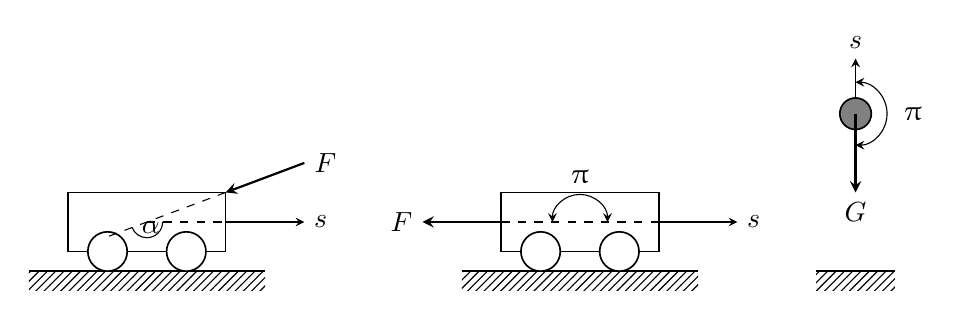
\begin{tikzpicture}[>=stealth,scale=1]
  \fill [pattern=north east lines](-1.5,-.25) rectangle (1.5,0);
  \draw [thick](-1.5,0)--(1.5,0);
  \draw [semithick](-1,.25) rectangle (1,1);
  \draw [semithick,fill=white] (-.5, .25) circle (.25);
  \draw [semithick,fill=white] (.5, .25) circle (.25);
  \draw[dashed] (0,1.25/2)--(1,1.25/2);
  \draw [->] (1,1.25/2)--(2,1.25/2)node[right]{$s$};
  \draw [dashed] (1,1)--(0,1.25/2)--(-.5, 1.25/2-0.375/2);
  \draw [thick,->] (2, 1+.375)node[right]{$F$}-- (1,1);
  \draw (0.2,1.25/2) arc (0:-160:.2)node[right]{$\alpha$};
  \begin{scope}[xshift=5.5cm]
    \fill [pattern=north east lines](-1.5,-.25) rectangle (1.5,0);
    \draw [thick](-1.5,0)--(1.5,0);
    \draw [semithick](-1,.25) rectangle (1,1);
    \draw [semithick,fill=white] (-.5, .25) circle (.25);
    \draw [semithick,fill=white] (.5, .25) circle (.25);
    \draw [dashed] (-1,1.25/2)--(1,1.25/2);
    \draw [thick,->] (-1,1.25/2)--(-2,1.25/2)node[left]{$F$} ;
    \draw [->] (1,1.25/2)--(2,1.25/2)node[right]{$s$};
    \draw [<->](0.35,1.25/2) arc (0:180:.35);
    \node at (0,1.2){$\uppi$};
  \end{scope}
  \begin{scope}[xshift=9cm]
    \fill [pattern=north east lines](-.5,-.25) rectangle (.5,0);
    \draw [thick] (-.5,0)--(.5,0);
    \draw [semithick,fill=gray](0,2.0) circle (.2);
    \draw [thick,->] (0,2.0)--(0,1.0)node[below]{$G$};
    \draw [->] (0,2.2)--(0,2.7)node[above]{$s$};
    \draw[<->] (0,1.6) arc (-90:90:0.4);
    \node  at (0.5, 2)[right]{$\uppi$};
  \end{scope}
\end{tikzpicture}
\end{document}